\documentclass[conference]{IEEEtran}

% -------------------------------------
% Packages
% -------------------------------------
\usepackage{cite}
\usepackage{amsmath,amssymb,amsfonts}
\usepackage{algorithmic}
\usepackage{graphicx}
\usepackage{textcomp}
\usepackage{xcolor}
\usepackage{dirtree}
\usepackage{comment}
\usepackage{acronym}
\usepackage{makecell} % used for cell creation in tables

%Darstellung von URL
\usepackage{url}
\urlstyle{same}
\usepackage{hyperref}
% -------------------------------------

% Set cell alignment default to vertial top and horizontal left
\renewcommand{\cellalign}{tl}
\renewcommand{\theadalign}{tl}

\def\BibTeX{{\rm B\kern-.05em{\sc i\kern-.025em b}\kern-.08em
    T\kern-.1667em\lower.7ex\hbox{E}\kern-.125emX}}



\begin{document}

\label{sec:title}
\title{Green Streaming Data Analytics Dashboards}

%\author{\IEEEauthorblockN{Christian Stubbe}
%\textit{TU Berlin} \\
%\textit{c.stubbe@campus.tu-berlin.de}

%\and

%\IEEEauthorblockN{Florian Baumann}
%\textit{TU Berlin} \\
%\textit{florian.baumann@campus.tu-berlin.de}

%\and

%\IEEEauthorblockN{Max Weßling}
%\textit{TU Berlin} \\
%\textit{max.wessling@campus.tu-berlin.de}

%\and
%\\
%\IEEEauthorblockN{Moustafa Ghaddar}
%\textit{TU Berlin} \\
%\textit{moustafa.ghaddar@campus.tu-berlin.de}
%}

\author{\IEEEauthorblockN{Christian Stubbe}
\textit{c.stubbe@campus.tu-berlin.de} \\
\IEEEauthorblockN{Florian Baumann} 
\textit{florian.baumann@campus.tu-berlin.de} \\
\IEEEauthorblockN{Max Weßling} 
\textit{max.wessling@campus.tu-berlin.de} \\
\IEEEauthorblockN{Moustafa Ghaddar}
\textit{moustafa.ghaddar@campus.tu-berlin.de} \\ \\

Technische Universität Berlin \\
Berlin, Germany
}


\maketitle
% To add page numbers:
\thispagestyle{plain}
\pagestyle{plain}


\label{sec:abstract}



\begin{abstract}

The widespread adoption of streaming services in our modern digital landscape has raised concerns about their environmental impact, particularly in terms of electricity consumption. As streaming continues to grow as a primary source of entertainment, it becomes imperative to address these environmental challenges. Our project aimed to tackle this issue by developing a content based measurement system that tracks electricity consumption per content played on streaming platforms. By providing streaming providers with insights into their energy usage, our system empowers them to better manage their environmental footprint and work towards sustainable streaming practices. It also allows researchers to experiment with the content and acquire deeper insights into the factors that play a major impact in energy consumption in the context of streaming. 

To achieve this objective, we implemented a web application capable of pulling data from a designated API (NETIO) and integrating it with CMCD. This combined dataset is then stored in a Postgres database and visualized using Grafana dashboards, allowing for comprehensive analysis of energy consumption patterns. Our system operates by establishing user sessions and collecting data during video playback, with CMCD providing valuable insights into content consumption behavior. Additionally, we utilize node-schedulers to periodically request data from NETIO devices, capturing baseline power consumption of playback devices.

The system also includes functionality for starting and stopping sessions, enabling users to initiate and terminate data collection as needed. Active sessions are monitored, and inactive sessions are automatically terminated after a specified period, ensuring efficient resource utilization.

The Grafana dashboard serves as a central hub for data visualization, aggregating session, CMCD, and energy consumption data. This comprehensive visualization platform empowers streaming providers to make informed decisions regarding energy consumption and environmental impact mitigation strategies. The Grafana dashboard was also implemented in a manner that allows the user to seamlessly alter the graphs and switch between multiple CMCD metrics along with the energy consumption depending on the interest of the user. In the concluding section of this report, limitations and further possible future improvements of the system are discussed. 

\end{abstract}
\label{sec:introduction}
\section{Introduction}

In today's modern digital landscape, streaming services and video on demand (VOD) has become an ubiquitous part of our daily routine. In fact, research show that, since 2017, only 12\% of the Swedish population exclusively watched traditional TV and in 2019, 22\% of the entire population did not consume content on traditional TV at all \cite{a2020_anvndning}. This data indicates a shift in the way the new and upcoming generations interact with online content and hints at the growing role that VOD will have in the near future. However, the environmental impact  and implications of such a technology, particularly in terms of electricity consumption, remain partly unknown. Reports indicate that the transmission as well as the processing of video content on the internet resulted in 306 million tons of carbon dioxide in 2018, which makes up nearly 1\% of the global greenhouse gas emissions \cite{efoui2019climate}. As data rates increase and internet service offerings improve, it is likely that the question around the carbon footprint of online video streaming will gain importance in the next few years. In fact, research shows that the carbon footprint of streaming decreased in the last few years, which is likely due to an increase in the efficiency of video coding standards as well as other technologies in the encoding, transmission and processing of video content. It is, however, still reasonable to assume that its carbon footprint will likely increase in the next few years as demand increases \cite{kamiya2020carbon}. Additionally, there is a lack of accessible and user-friendly tools and software that provide an insight into the energy consumption of streaming. The objective of this project is to develop a content-based measurement system that monitors electricity usage per content played on streaming platforms. This system will empower streaming providers to gain insights and effectively manage their environmental footprint, fostering a more sustainable approach to streaming.



\label{sec:related_work}

\section{Related Work}
In data streaming analytics applications, there are very few products available on the market, each presenting their own benefits and disadvantages for different use-cases in the industry such as online learning or sports streaming. Each data analytical system is usually accompanied with other services such as video encoding, hosting and delivery. Firstly, one of the most popular products in the market is \textbf{api.video} \footnote{api.video: https://api.video/}, which is a service that allows users to collect real-time play event data for live streams and videos and display them. However, the data collected is shallow and limited to the client's attributes such as the device type, the operating system, browser and approximate location. In-depth analytics, such as power consumption, are not available and other data aggregations are not performed. However, these aspects should not be ignored as research indicates that the client-side energy consumption is indeed the most significant. In fact, the International Energy Agency reports that consumer devices account for 72\% of the energy used for streaming \cite{kamiya2020carbon}. 

Secondly, in terms of applications that are not limited to video streaming but any kind of data streams, there exist many products and frameworks that offer this service such as Apache Flume, Spark streaming, Storm, Apache Flink, Kafka streams and many others. Qualitative research highlights the fact that these applications and frameworks are difficult to operate and expensive, leaving customers not satisfied with the product \cite{chimariya2018streaming}. 

The previous examples all show that there is a market gap for a simple solution that allows the streaming provider to get a better overview of the environmental impact they are having. Such a system is also useful for research such as testing the efficiency of different adaptive bitrate streaming (ABR) algorithms and, therefore, would be targeted at the researchers as opposed to consumers. 

\label{sec:approach}

\section{Solution Approach}
%The approach that was taken for this project was...
\begin{comment}
Given task
- build a video player able to change playback settings (bitrate, ...) 
- collect CMCD data during playback of videos
- collect energy consumption data from playback device via Netio smart power plugs
- combine and analyse data in Grafana dashboards

first approach
- get familiar with the technology \& develop architecture (workshop 1)
- 

changes during development process
- simplified architecture 


- Grafana dashboard (Max)
    different diagramms: .... TODO
- everythin in docker (Max)
    
\end{comment}
\begin{comment}
problems we had:
- requesting netio data: concurrency -> from setTimeout to node-scheduling ( aspect: get the resting power consumption of the device when no video is played to be able to normalize the data)
- store the video data -> TUBCloud to example video files on dash website (no storing in the git repo, no downloading for the user, easy access)
- creating the session id in the frontend -> not best practice (theoretically, the id can be assigned twice)
- exposing the netio device to the internet
- baseline energy consumption of devices
\end{comment}

%\subsection{Overall Architecture and running tests}
Our application is structured around five main components, each playing a crucial role in the data collection and analysis process.

\subsection{Component Overview}

\subsubsection{Netio Device} At the foundation of our data collection process is the Netio power socket, a device capable of measuring the energy consumption of connected electronic devices. 
It collects detailed energy usage data and makes this information accessible via an endpoint on the local network. 
By interfacing directly with our application, the Netio device provides power consumption metrics essential for our analysis.

\subsubsection{Media Player Frontend} The media player frontend is where the interaction with the user takes place. 
Through the media player interface, users can input Netio device data, control video playback, and conclude measurement sessions, making it a critical component of our system.

\subsubsection{Measurement Server} Serving as the application's main backend, the measurement server has multiple interfaces connecting it to the other components. 
It is responsible for receiving Client Media Common Data (CMCD) from the frontend, which contains valuable information about the video playback. 
Additionally, it requests energy consumption data from the Netio device and stores all collected data in the database. 
This centralized server is in managing data flow and ensuring the integrity and reliability of the data collected.

\subsubsection{Database} The database is the repository for all relevant data collected during the measurement sessions. 
It stores energy consumption data, CMCD, and session data that is crucial for analysis. 
This structured data storage allows for efficient data retrieval and analysis, serving as the foundation for generating insights into energy consumption patterns on the dashboards.

\subsubsection{Grafana Dashboards} To visualize and analyze the collected data, we employ Grafana dashboards. 
These dashboards are designed to aggregate the data from our database, presenting it in an intuitive and informative manner. 
By correlating power consumption data with CMCD, the dashboards provide insights into the relationship between video playback characteristics and energy usage. 
This visual analysis tool is useful for identifying patterns and drawing conclusions from the collected data.

In the subsequent sections, we will offer detailed insights into the frontend, backend, and Grafana dashboards, providing a deeper understanding of the internal processes. A diagramm showing the components, processes and data flows can be found in the appendix \ref{fig:project_architecture}.

\subsection{Frontend: Media Player }
Our web application's frontend is engineered to deliver an efficient user experience, enabling testing of video playback scenarios and collection of CMCD. 
This entails a sequence of user interactions and system responses. 
The frontend was developed using Vue.js with Typescript and Vuetify as the framework. It provides an engaging platform for users to execute their measurements, which are outlined through a series of steps:

Users launch the application by navigating to its URL in the web browser installed on their Smart TV, laptop or PC. 
Upon accessing the frontend, users are prompted to enter the configuration data for the Netio power socket, including the IP address and password. 
This information is crucial for establishing a communication link between the application and the Netio device. 
With the Netio settings configured, the application generates a unique session UUID. 
This identifier is crucial for correlating the collected power data with the specific session and later the CMCD. 
The session UUID is subsequently sent to the backend, marking the beginning of the data recording phase (a session). 
Users can then start the video playback. 
During playback, Client Media Common Data with the session ID which is stored in a cookie is sent to a designated endpoint in the backend. 
This data includes key metrics relevant to the playback performance. Throughout the testing session, users retain control over the playback. They have the option to pause the video, resume playback, or switch to a different video, depending on the testing requirements.

The session can be concluded in two ways. Users can manually end the session by clicking the "End Session" button within the application. 
Alternatively, the session will end after a set period of inactivity.

For video playback, we have opted to host our video files on Google Cloud for reliable and scalable access to the video content. The videos were encoded locally before being uploaded, allowing users to choose the playback quality and ensuring adaptive bitrate streaming (ABR).

\subsection{Backend: Measurement Server and Database}
The backend of our web application is a critical component designed to manage sessions, collect the energy consumption data, and ensure seamless communication between the frontend and the database. 
Our tech stack comprises a Node.js server with Express and a PostgreSQL database that includes tables for "sessions", "cmcd", and "netio". This setup provides a robust and efficient platform for data management and retrieval.

The interaction between the frontend and the backend begins when the frontend submits the first request containing the session ID and the Netio device configuration data. 
This POST request triggers the creation of a new session entry in the database, effectively initializing the test session.
Subsequently, the frontend starts sending Client Media Common Data to the backend when playing a video, targeting the designated endpoint. 
This CMCD, which includes information about the video playback on the client, is stored in the "cmcd" table, along with the corresponding session ID. 
This structured approach ensures that all collected data is accurately associated with its respective session, enabling detailed analysis in the Grafana dashboards.

To efficiently collect Netio power consumption data, we employ node-scheduler to execute periodic tasks.
This scheduler triggers a function every 10 seconds, tasked with identifying active sessions by querying the "sessions" table. 
Upon identifying an active session, the function retrieves the Netio device configuration using the authentication data stored alongside the session information. 
The collected Netio data is then stored in the "netio" table, associated with the respective session ID.
This method allows for the simultaneous monitoring of multiple Netio devices without encountering issues related to parallel processing on the Node.js server.

In addition to collecting Netio data, another critical function of our backend involves monitoring session activity. 
Using node-scheduler, the system checks every minute for sessions that have not received CMCD for the past 30 minutes. 
Such sessions are flagged as terminated in the database, indicating that data collection for those sessions has concluded. 
This automated process ensures that sessions are accurately tracked and managed, allowing for the efficient termination of inactive sessions and the conservation of resources.

\subsection{Grafana Dashboards}
For the display and visual analysis of the gathered data, two separate dashboards were developed for the open-source visualization web application Grafana \footnote{Grafana Labs: https://grafana.com/}.

\subsubsection{Overview dashboard}
The first dashboard provides concise information about the existing sessions. Besides the total number of currently active sessions, a table lists all existing sessions along with descriptive attributes such as the session creation time, the IP address and the serial number of the associated Netio device, and the time the last CMCD entry was received. It serves as the entrypoint of the dashboard ensemble and is used to identify the sessions that should be inspected further.

\subsubsection{Session-specific dashboard}
The second dashboard is a session-specific dashboard that displays detailed data from a selected session. A filter on the very top of the dashboard can be used to select a session. In the upper part of the dashboard, a table displays the metadata attributes for the selected session.

The next part of the dashboard focuses on energy consumption data. A line graph shows the baseline load, the total load, and the total load minus the baseload load captured during the selected session in watts over time. The baseline load is calculated in an attempt to then distinguish the playback device’s energy consumption while idling from its energy consumption during video playback. To achieve this, the arithmetic mean of the energy consumption of the playback device before the first CMCD entry was created is considered the baseline load. The creation time of the first CMCD entry is used as a proxy for the video playback start as this marks the point in time when the first video segment was requested by the playback device.

The aforementioned energy consumption visualization is combined with different CMCD metrics in the following parts of the dashboard. By default, three line graphs show the energy consumption data together with the measured throughput between the client and the content server, the video’s bitrate, and the buffer length, respectively. Another graph shows the energy consumption data along with a user-selected CMCD metric. This allows the user to analyze the captured data in a flexible manner. (possible selections: bitrate, buffer length, duration, deadline, measured throughput, playback rate, requested maximum throughput, top bitrate.

\subsection{Dockerization}
Dockerization played a pivotal role in ensuring the fast, reliable, and platform-independent shipment of our project components. By creating Docker container configurations for each component, we were able to encapsulate the environment in which our application runs. This encapsulation guarantees that our application works uniformly across any platform supporting Docker. All necessary components were integrated within one Docker compose file \footnote{The Docker compose file of our project: \url{https://github.com/florian-baumann/awt_ws2324/blob/main/src/docker-compose.yml}}. This approach not only simplified the development process, but would also serve as a ready-to-use method to operationalize the application. The utilization of environment variables, which are loaded during startup, enhanced our application's configurability and security. By externalizing configuration details to environment variables, we made our application adaptable to different environments without requiring changes to the codebase. This Dockerization strategy has been instrumental in ensuring that our application remains agile, portable, and easy to manage across diverse development and production landscapes.

\subsection{Running measurements}
Before initiating the measurement process, users must ensure they have the appropriate hardware and setup conditions. This involves mainly:
\subsubsection{Hardware Requirements} The measurement process is designed to be conducted on a Smart TV, a Laptop or PC. These devices should be capable of running a modern web browser, which is essential for accessing the Vue.js-based frontend of our application and playing videos.
\subsubsection{Power Connection through Netio Power Socket} The playback device must be connected to an electrical outlet via a Netio power socket. This setup is crucial for monitoring and recording the power consumption data accurately during the video playback.
\subsubsection{Optimizing the Measurement Environment} To minimize any potential interference with the power data collection, users are advised to terminate any unnecessary programs running on the device. The only application that should remain active is the web browser that runs our application.\\

\label{sec:evaluation}
\section{Evaluation}

The following section will present and discuss the results of the preliminary data collection. Furthermore it will critically evaluate the architectural decisions that were made during the design of the testing environment and the chosen tech stack. 

% -------------------------------------
\subsection{Preliminary Data Collection}
% -------------------------------------
As part of this project a preliminary data collection was conducted. For this preliminary data collection four hardware devices were used. The first device, a local machine, hosted the measurement server, the media player and the Grafana dashboards. The second device, a desktop PC, accessed the media player provided by the first device to playback videos. This desktop PC ran Windows 11 with a Ryzen 7 3700X CPU, an AMD RX5700XT GPU, and 32GB of RAM. The third device was an external monitor connected to the desktop PC. The external monitor was an Acer Nitro VG240YU with an WQHD resolution of 1440p. The fourth device was the Netio PowerCable 24A42C38E7EA. 

\begin{table}[ht]
\begin{tabular}{lll}
\hline
\thead{Device} & \thead{Task} & \thead{Technical Details} \\
\hline\hline
Local Machine &  \makecell{Provide \\ test environment} & \makecell{not relevant \\ for energy consumption} \\
Desktop PC & \makecell{Control \\ media player} & \makecell{ Windows 11 \\ CPU: Ryzen 7 3700X \\ GPU: AMD RX5700XT \\ RAM: 32GB} \\
External Monitor & \makecell{Display \\ media player} & \makecell{Acer Nitro VG240YU \\ WQHD 1440p} \\ 
Netio Device & \makecell{Measure \\ energy consumption} & ID 24A42C38E7EA \\ [1ex] 
\hline \hline
\end{tabular}
\vspace{.2cm}
\label{tab:data-collection}
\caption{Hardware devices used for preliminary data collection}
\end{table}

The Netio device captured both the energy consumption of the desktop PC and the external monitor. The external monitor was connected to the desktop PC via a DisplayPort cable. The energy consumption of the local machine running the measurement server, media player and Grafana dashboards was not measured as it is not relevant to the research question. Prior to the preliminary data collection, all background tasks that were not required were terminated on the desktop PC. The video was playing in full-screen. The display brightness was set to 100\% on the external monitor. 

As described in section \ref{sec:approach}) separate sessions for each video were created. Each section included 60s base load measurements before the first video segment was loaded in order to simplify the attribution of additional energy consumption during video playback to the research question. After this 60s base load period, the actual playback was started by using the “Start Session” button in the media player. 

The results of the data collection are part of the GitHub repository in the Grafana dashboards. The main task in this project is not to collect data, but to provide an adequate testing environment for further data collection. Hence, this evaluation will discuss the testing environment and not the results of the preliminary data collected itself in detail. 

% -------------------------------------
\subsection{Improvement of the preliminary data collection}
% -------------------------------------
The preliminary data collection can be improved by the following suggestions to increase the quality of the data collected: 

\begin{itemize}
  \item Mitigate the impact of background processes on the desktop PC
  \item Measure energy consumption of external monitor and desktop PC separately 
  \item Measure energy consumption of a variety of differences devices 
  \item Standardize the testing procedure
\end{itemize}

Healthy Windows systems will have a multitude of processes running in parallel. Each of theses processes influences the energy consumption. An improved data collection process should aim to minimize the impact of these processes on the energy consumption of the desktop PC. Furthermore, the energy consumption of the external monitor and the desktop PC should be measured separately. This allows to separate changes in the stream that are attributed to e.g. network traffic and CPU usage from changes in video brightness. Also, the energy consumption should be measured on a variety of different device categories and different devices within the same device category. As 60.3\% of households in Germany in 2022 had an internal-enabled television set (smart TV) \cite{medienanstalten2020}, the device category SmartTV should be measured next to desktop PCs. This would allow to gain more insights on the research question. Within one device category, measurements should be performed on multiple devices in order to mitigate any device-specific fluctuations in energy consumption that cannot be mitigated by reducing the number of processes running in parallel. As a last item, the testing procedure could be standardized in a document specifying the 60s base load period, the video in which videos are played and any interactions executed by the researcher on the media player e.g. adjusting video quality or sound. 

These changes in the data collection would lead to more fine-grained energy measurements and allow a more sophisticated analysis. Ultimately in a perfect testing environment each segment request should be related to a spike in energy consumption and can be deconstructed into energy consumption caused by the network traffic, the monitor and the playback of the video itself. 

% -------------------------------------
\subsection{Evaluation of available features}
% -------------------------------------
This section will critically discuss the user flow in the testing environment. 

As described in section \ref{sec:approach} the media player creates a new session ID as soon as the user enters the Netio device configuration. This leads to the risk of ID collision, which could lead to confusion when analyzing the data in the Grafana dashboards. The session ID is generated with UUIDv4 as a random value of 122 bits leading to $2^{122}$ possible values. This translates into a 50\% chance of generating a single collision when 1 billion v4 UUIDs are generated for 85 years. Due to these odds, the generation of the session ID in the media player is unlikely to have any impact on the quality of the data collection. 

In its current state the testing environment only supports dash.js. Depending on the research question, playing videos with HLS might be relevant as well. This would require only minor changes to the media player. The measurement server is  already player-agnostic to support an HLS player. 

The testing environment is designed to be used by multiple Netio devices in both a single network or across multiple networks. In a multi-network scenario the Netio device needs to be exposed to the public internet in order to communicate with the measurement server. As the current setup supports a variety of data collection scenarios, it is possible to fulfill the suggested measurements across a variety of differences devices in device categories, as described in the previous subsection. 

% -------------------------------------
\subsection{Evaluation of the technology stack}
% -------------------------------------
This section critically evaluates the use of Node.js, Vue.js, PostgreSQL, and Docker as a combined technology stack for the testing environment. A detailed overview of the usage of these technologies in the project was presented in section \ref{sec:approach}. All languages, frameworks and tools in the technology stack are well-established. JavaScript is the the most popular programming language in the world \cite{jetbrains2023} and Vue.js is with 32\% of JavaScript developers using it, the second most-used JavaScript framework after React.js. Node.js is being used on more than 6.3 million websites, including popular sites such as Cloudflare, GitHub and Spotify \cite{Radixweb2023}. This makes Node.js also likely a solid choice for the foreseeable future. PostgreSQL has become the most admired and desired database in the 2023 Stack Overflow survey \cite{StackOverflow2023}. However, MySQL reaches under extreme-write workloads a slight advantage over PostgreSQL \cite{Bytebase2023}. But this scale is not relevant for this project. Furthermore PostgreSQL is released under a very liberal Open Source license comparable to the MIT license, while MySQL is owned by Oracle \cite{Bytebase2023}. In the 2023 Stack Overflow Docker was ranked as the most-used developer tool \cite{StackOverflow2023}. Due to these usage statistics, the combined use of Node.js, Vue.js, PostgreSQL, and Docker presents a robust technology stack for the testing environment. 
\label{sec:conclusion}

\section{Conclusion}

The main objective of this project is to tackle the issue of green streaming by developing a content based measurement system that tracks energy consumption per content played and displays the aggregated data on a dashboard. It can be concluded that the main goal of this project was achieved along with its deliverables, which include 

The main goal of this project was achieved, as we successfully developed a content-based measurement system to address the issue of green streaming. Our system effectively tracks energy consumption per content played and presents the aggregated data on intuitive Grafana dashboards. By accomplishing this objective, we have taken significant steps towards promoting sustainability in the streaming industry as well as aiding with green streaming related research .

In addition to achieving our main purpose, we have successfully delivered the following key deliverables:

\begin{enumerate}
  \item Player Application: A user-friendly application that enables users to access and play demo videos, facilitating seamless interaction with the streaming platform \ref{fig:media_player1} \ref{fig:media_player2}.
  \item Backend Server: An efficient backend server that collects energy consumption data and stores Common Media Client Data (CMCD), ensuring the reliable storage and management of essential metrics.
  \item Grafana Dashboards: Comprehensive dashboards developed using Grafana, allowing stakeholders to analyze energy consumption data alongside CMCD metrics. These dashboards provide valuable insights into streaming patterns and energy usage, empowering decision-making processes \ref{fig:dash1} \ref{fig:dash2}.
\end{enumerate}

With these deliverables in place, our project has not only achieved its primary objective but has also provided tangible tools and resources to support ongoing efforts towards green streaming. We are confident that our system will contribute to greater awareness and accountability in the streaming industry, ultimately leading to a more sustainable future.
\label{sec:acknowledgements}

\section*{Acknowledgements}

We would like to express our sincere gratitude to the \textbf{Fraunhofer FOKUS} institution for their support, which made this project possible. Special thanks to our supervisors, Ahmed Amine Mchayaa, Robert Seeliger, and Stefan Pham for their valuable guidance, support, and insightful feedback throughout the research process. Additionally, we extend our appreciation to our professor Louay Bassbouss, for his collaboration and constructive discussions. This project has truly been a collaborative effort, and we are thankful for the encouragement and assistance received from our peers. 



\bibliographystyle{ieeetr}
\bibliography{references}

\cleardoublepage
% \addcontentsline{toc}{section}{Appendices}
\onecolumn
\appendix
\begin{appendices}
%\addtocontents{toc}{\protect\setcounter{tocdepth}{0}}

\section{Grafana dashboard}
\label{dash1}

\begin{figure}[ht]
    \centering
    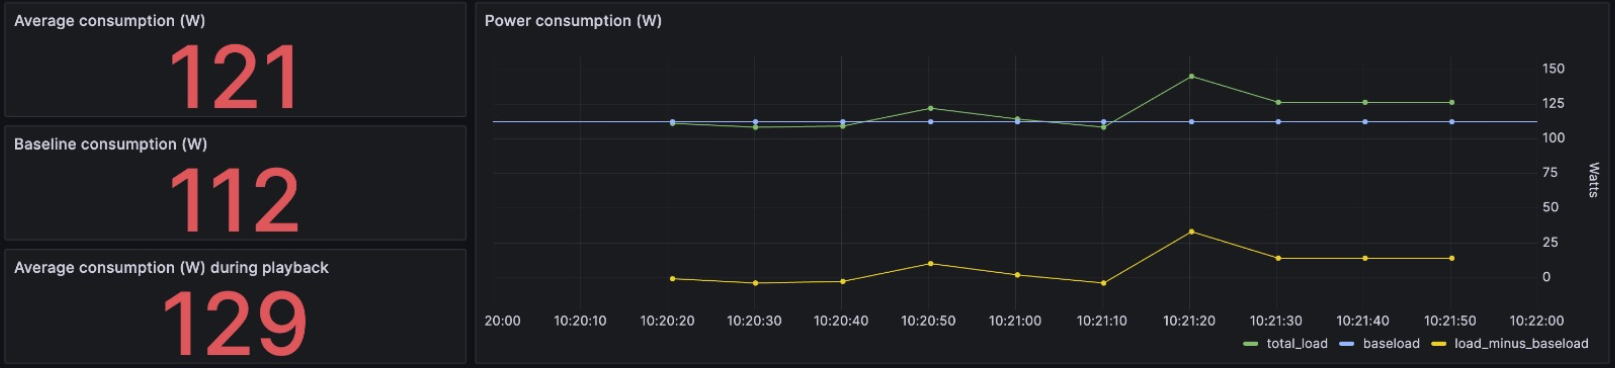
\includegraphics[width=1\linewidth]{assets/dashboard1.png}
    \caption{First graph of the Grafana dashboard}
    \label{fig:dash1}
\end{figure}

\begin{figure}[ht]
    \centering
    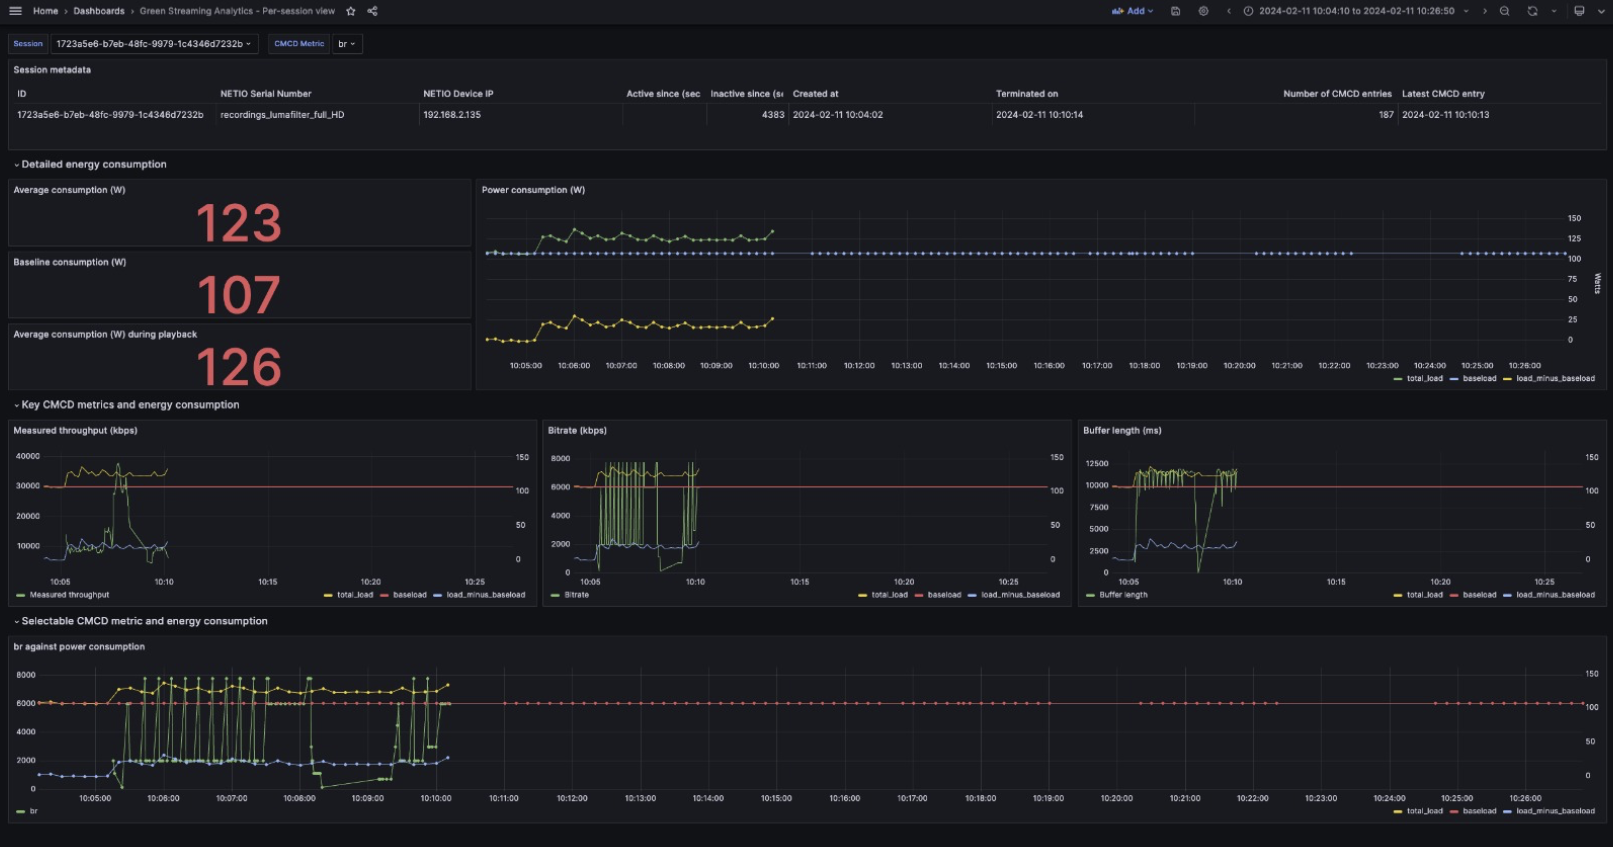
\includegraphics[width=1\linewidth]{assets/dashboard2.png}
    \caption{Second graph of the Grafana dashboard}
    \label{fig:dash2}
\end{figure}

\section{Player Application}

 \begin{figure}[ht]
     \centering
     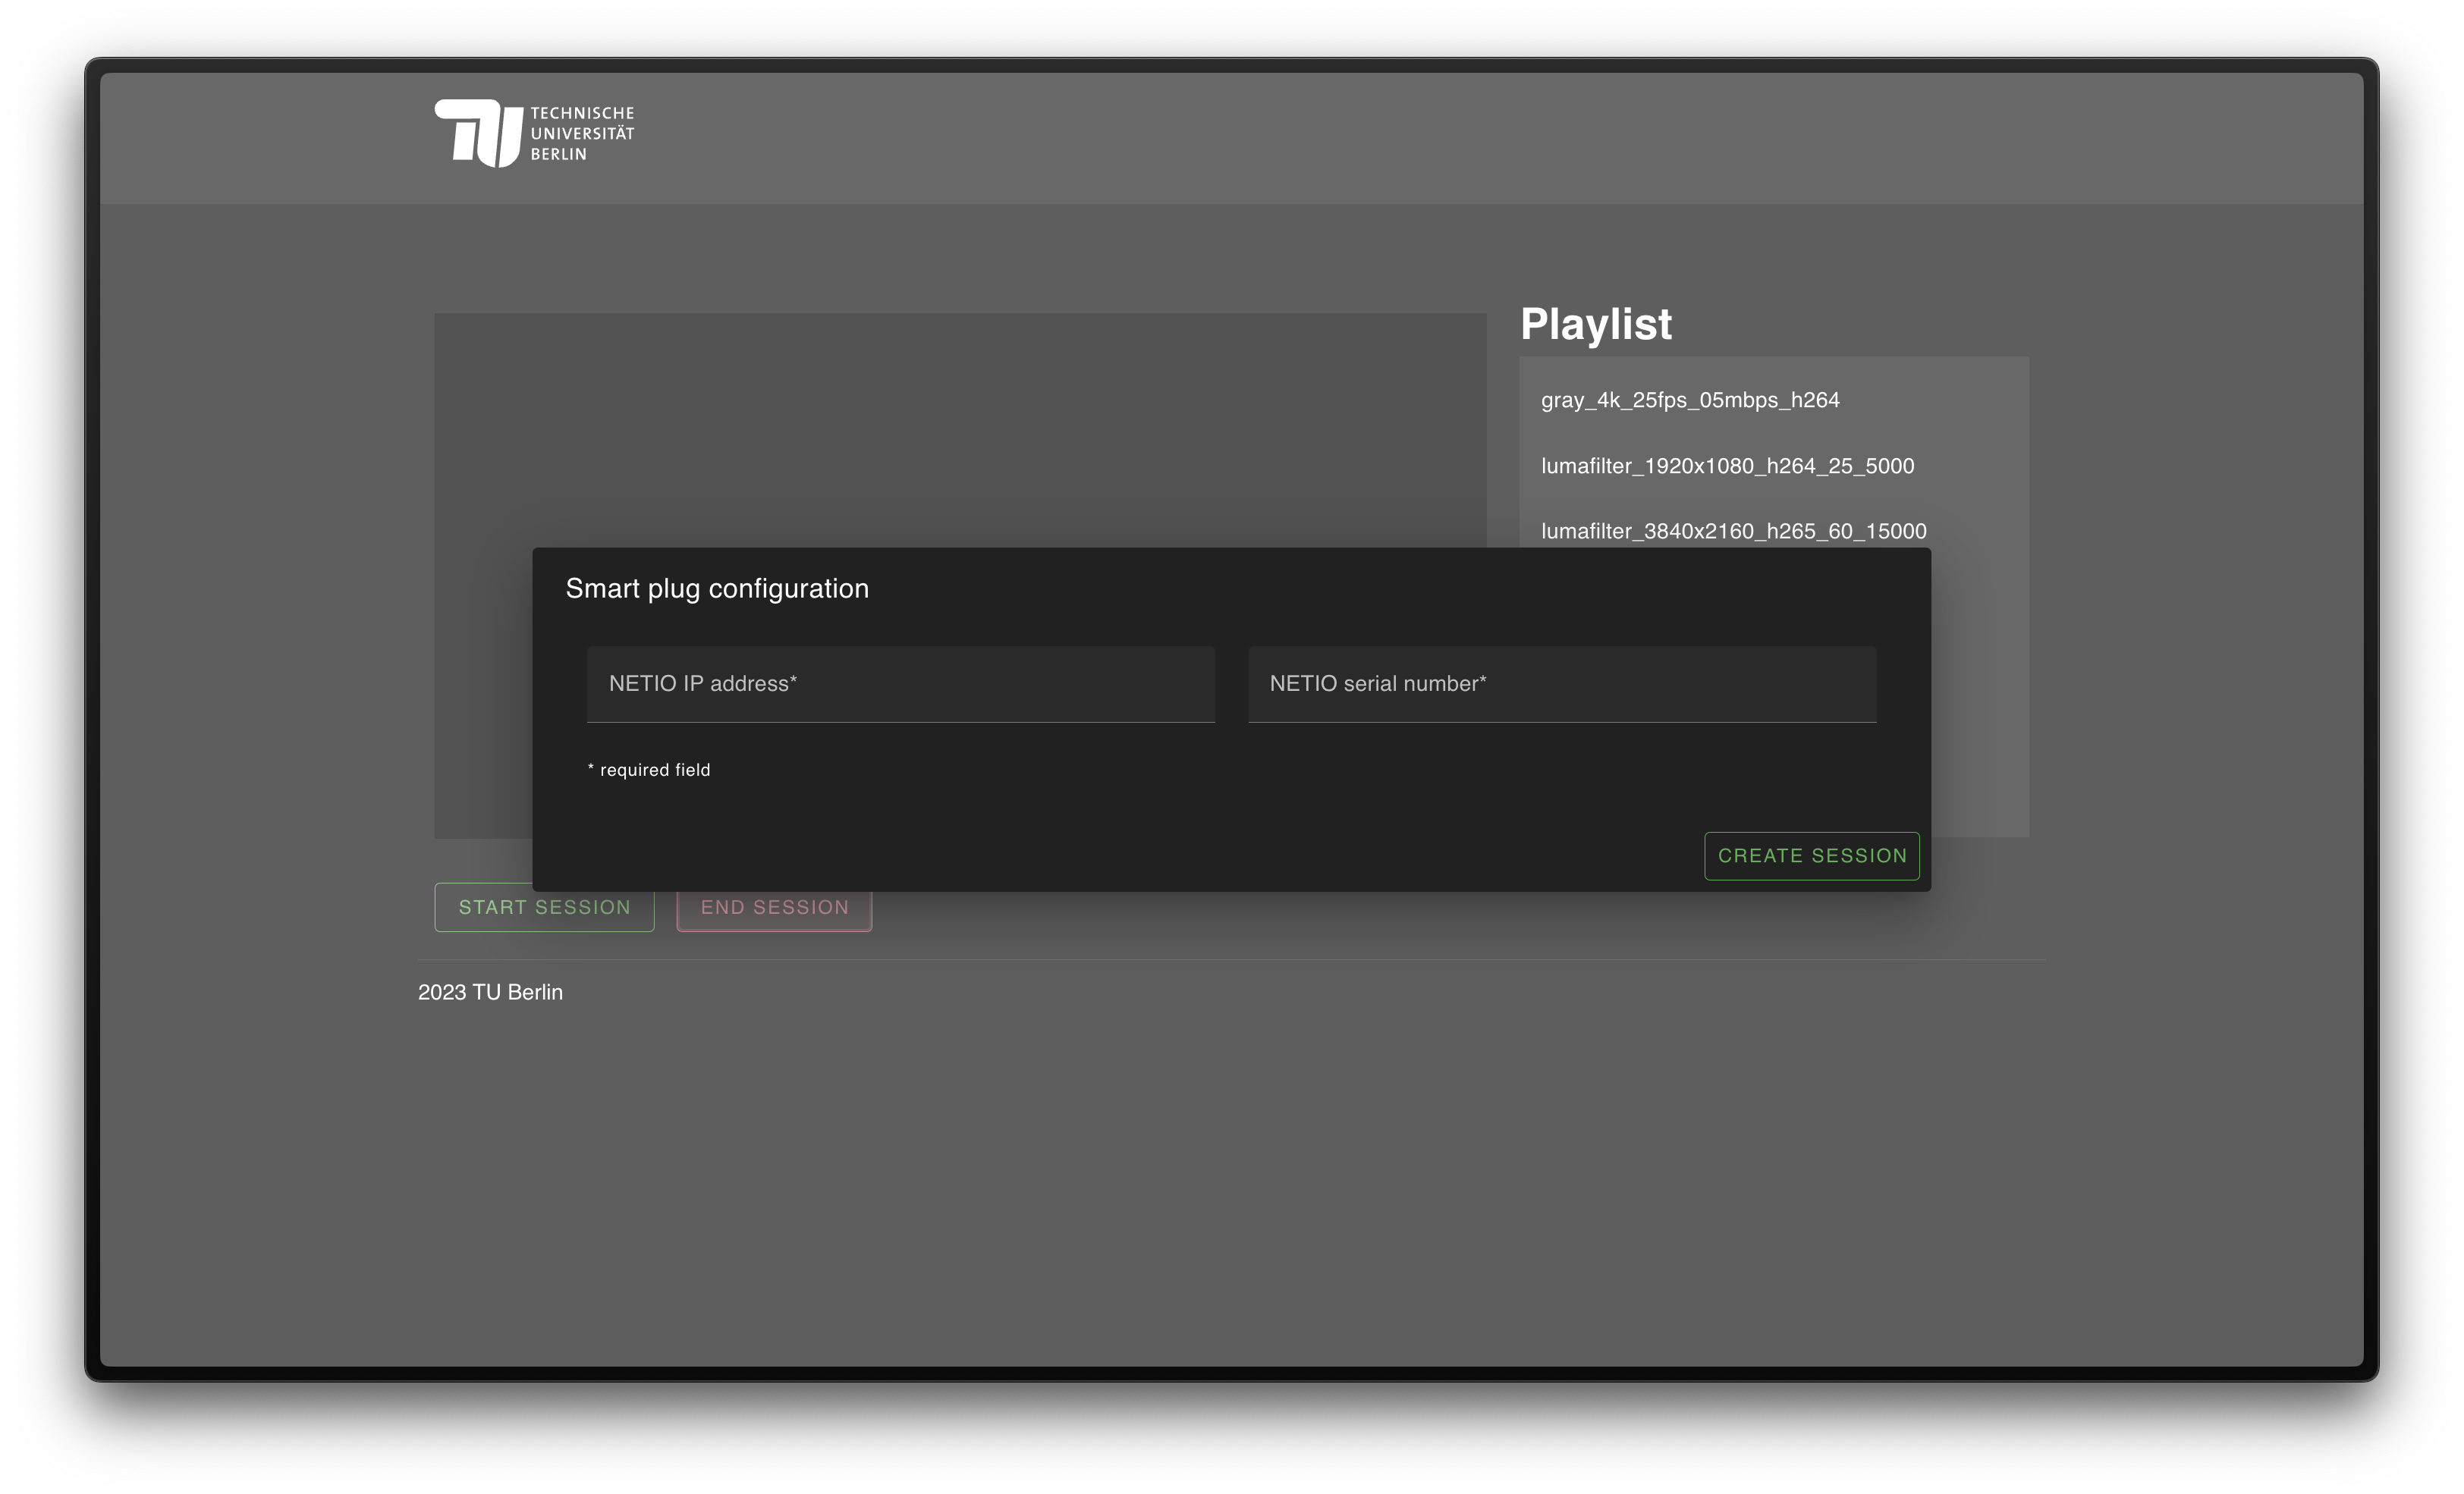
\includegraphics[width=0.8\linewidth]{assets/mediaplayer1.png}
     \caption{The landing page of the frontend application.}
     \label{fig:media_player1}
 \end{figure}

 \begin{figure}[ht]
     \centering
     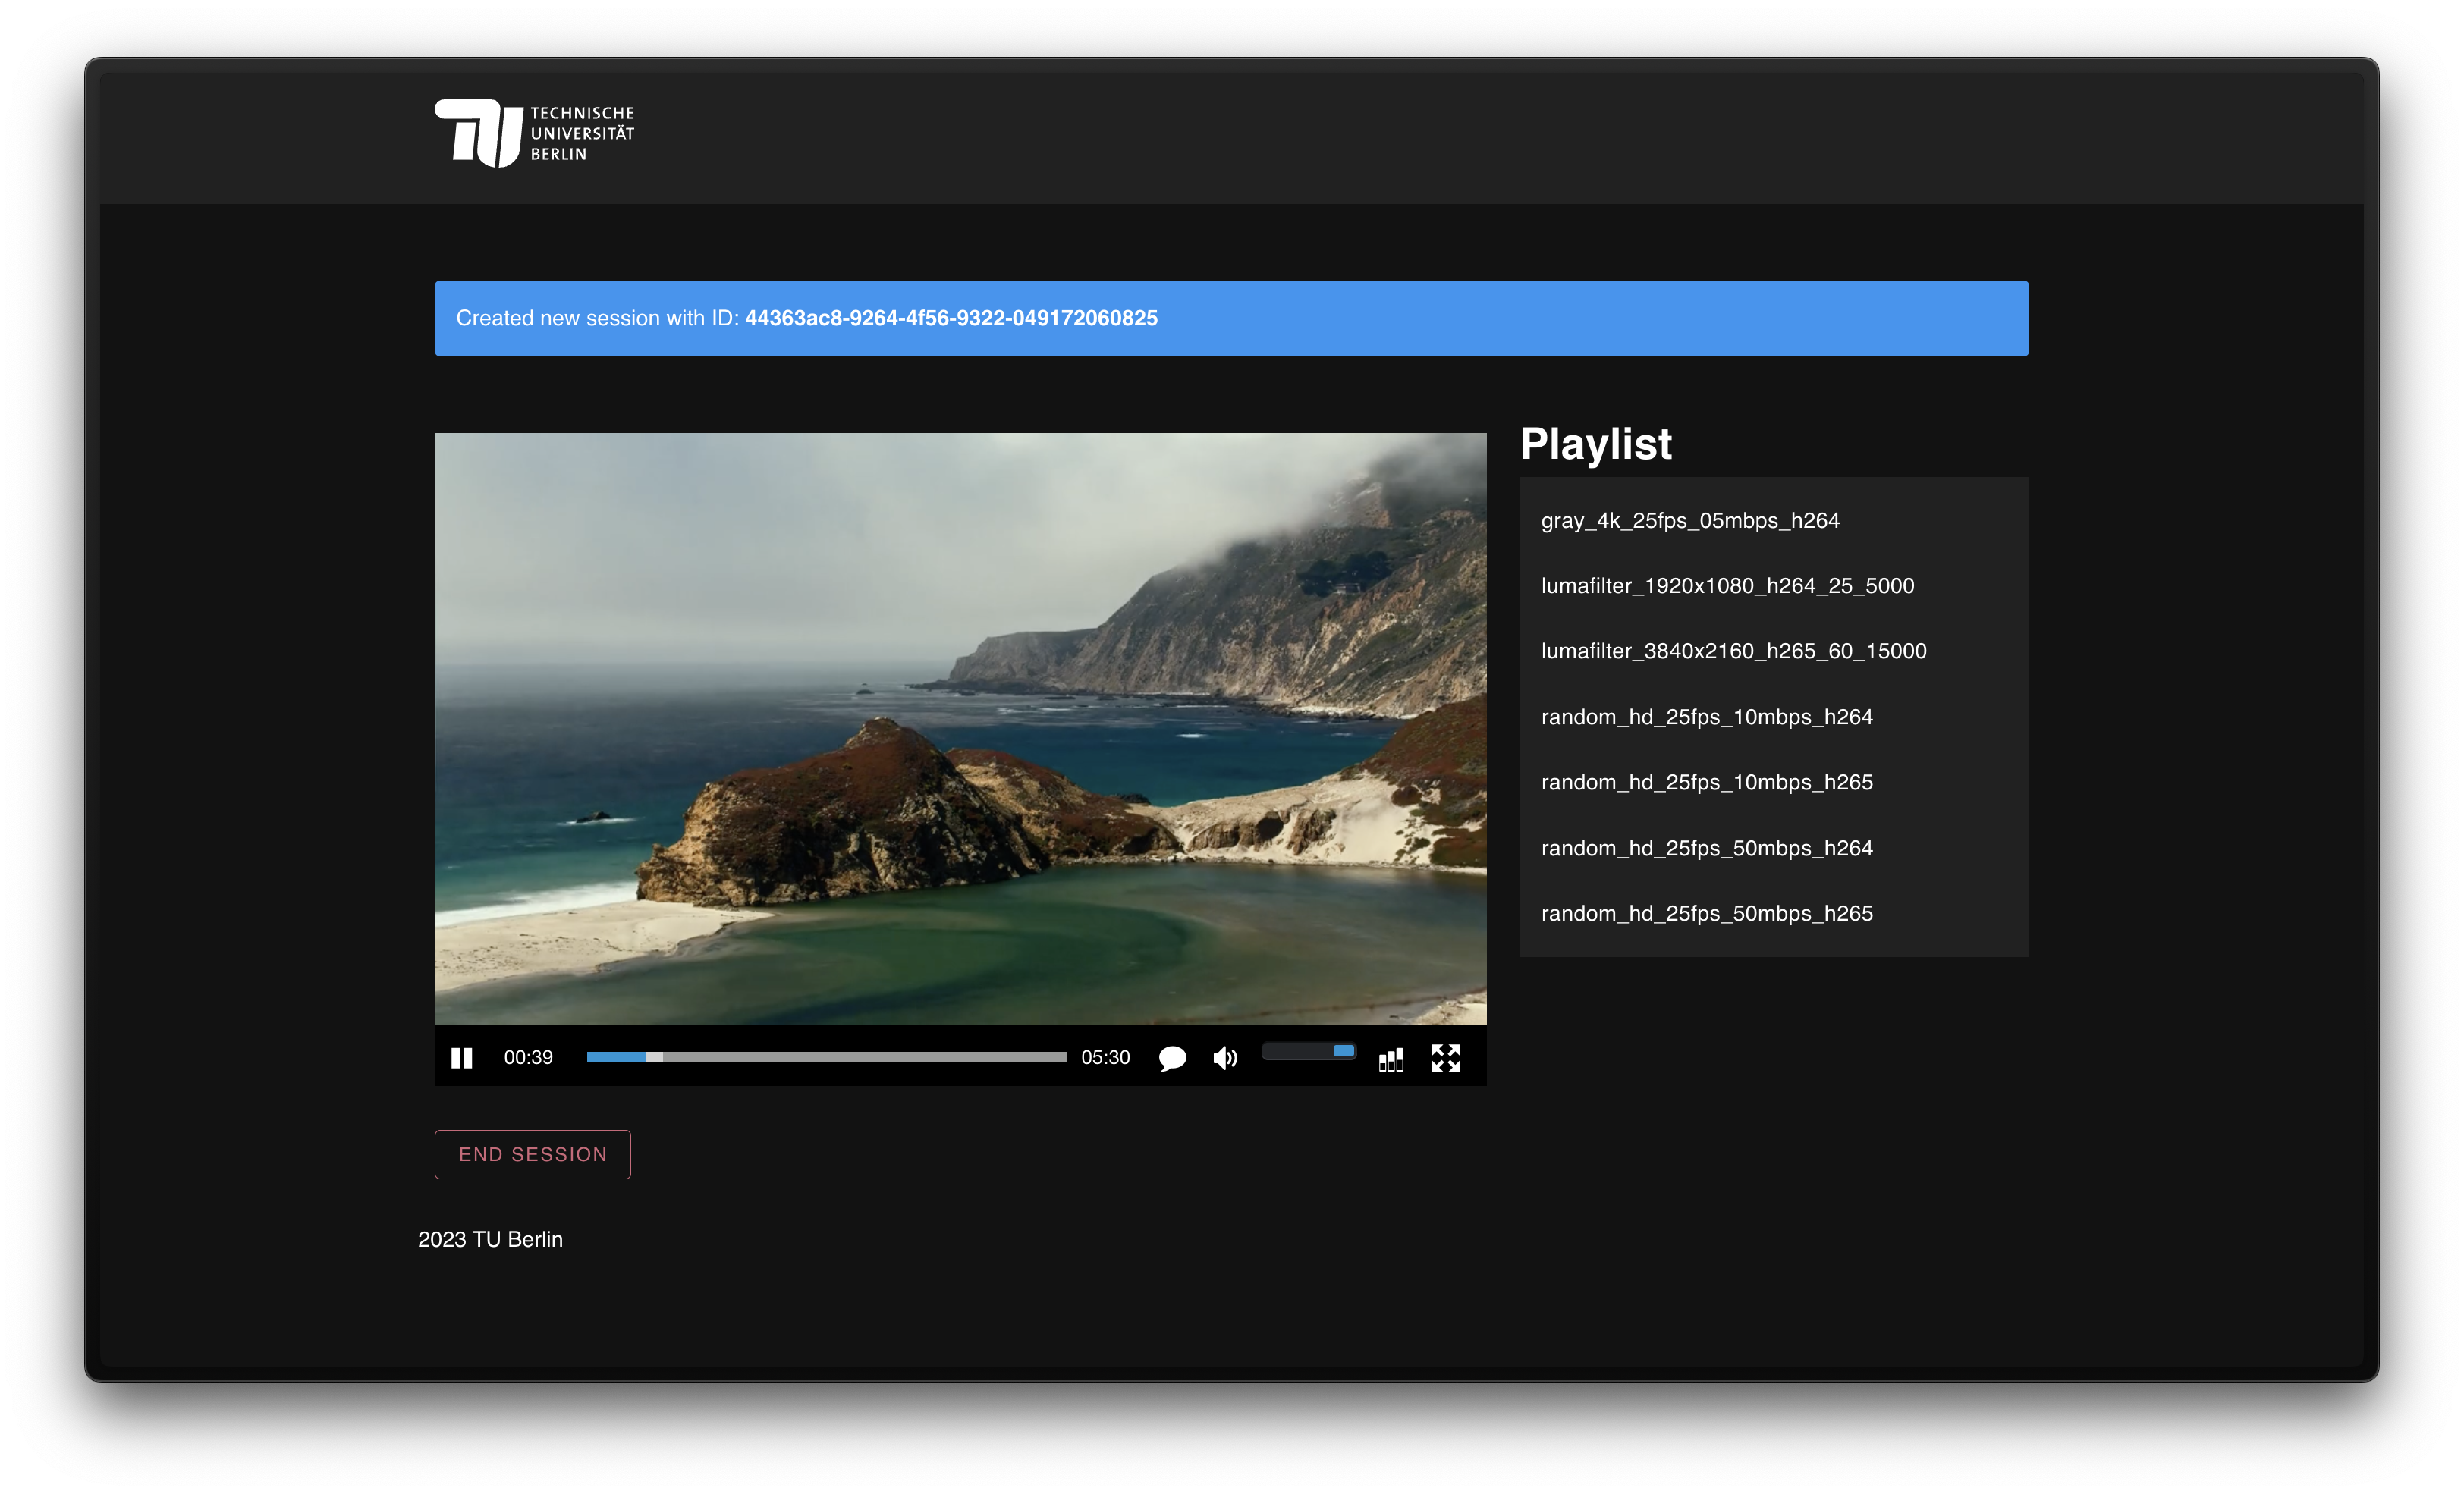
\includegraphics[width=0.8\linewidth]{assets/mediaplayer2.png}
     \caption{The frontend page of the application with the playlist and the player.}
     \label{fig:media_player2}
 \end{figure}

\section{Overall architecture}

 \begin{figure}[ht]
     \centering
     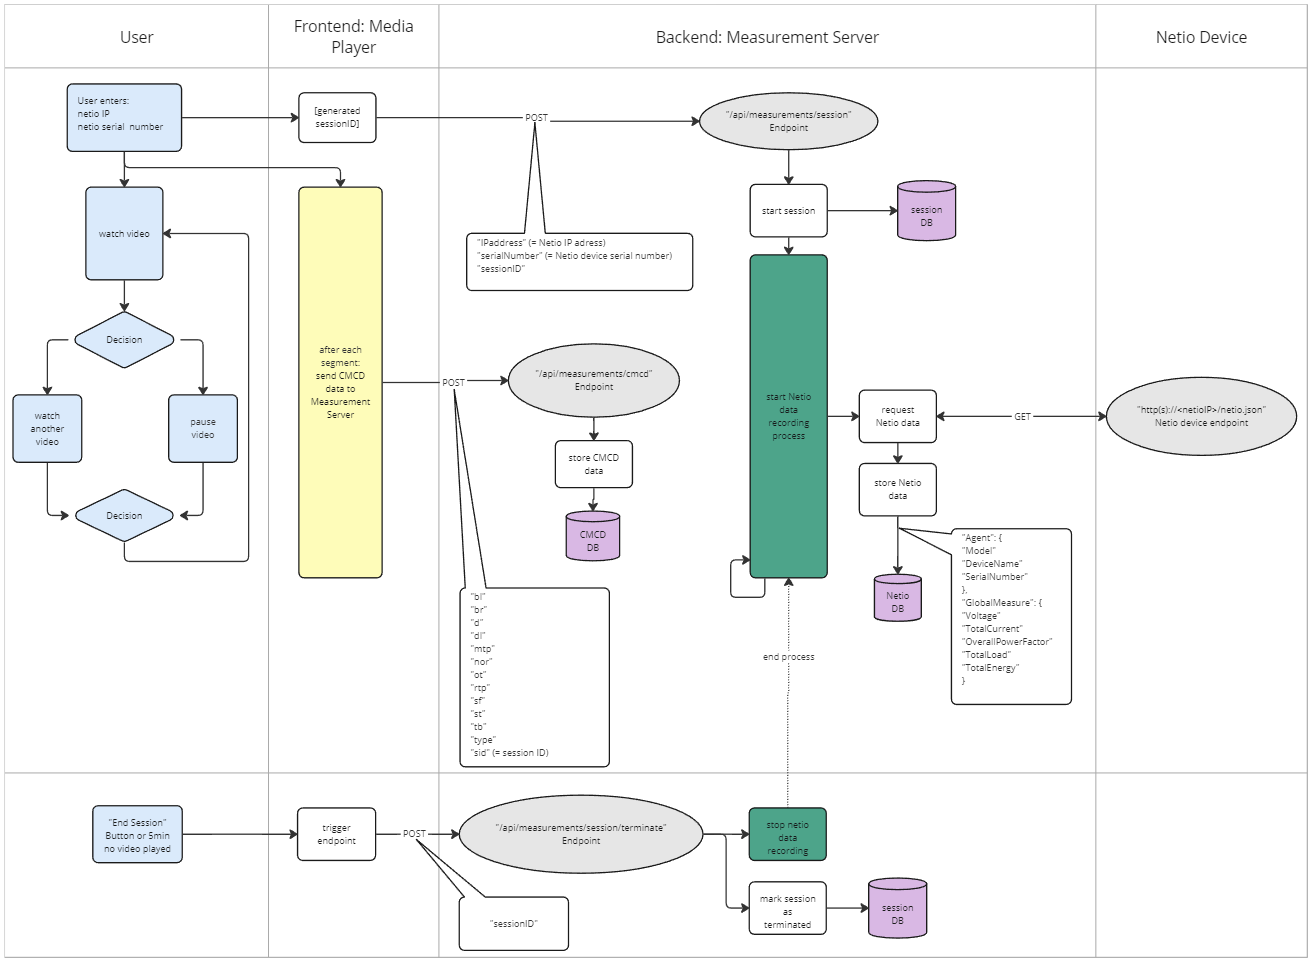
\includegraphics[width=1\linewidth]{assets/architecture_diagram.png}
     \caption{The overall architecture and internal process of the project.}
     \label{fig:project_architecture}
 \end{figure}


\section{Source Code}
% File Structure
    \begin{figure}[ht]
        \dirtree{%
        .1 green-streaming-analytics.
            .2 assets.
                .3 (...).
            .2 src.
                .3 grafana.
                    .4 data.
                        .5 (...).
                    .4 details-dashboard.json.
                    .4 docker-compose.yml.
                    .4 overview-dashboard.json.
                .3 measurement-db.
                    .4 init.
                        .5 init.sql.
                    .4 .gitignore.
                    .4 Dockerfile.
                    .4 sample-data-database-dump.sql.
                .3 measurement-service.
                    .4 config.
                        .5 config.js.
                    .4 controllers.
                        .5 cmcdController.js.
                        .5 sessionController.js.
                    .4 exampleData.
                        .5 netio.json.
                    .4 models.
                        .5 Cmcd.js.
                        .5 Netio.js.
                        .5 Session.js.
                        .5 index.js.
                    .4 services.
                        .5 (...).
                    .4 Dockerfile.
                    .4 index.js.
                    .4 package-lock.json.
                    .4 package.json.
                .3 media-player.
                    .4 src.
                        .5 assets.
                        .5 components.
                        .5 router.
                        .5 views.
                        .5 App.vue.
                        .5 main.ts.
                    .4 Dockerfile.
                    .4 index.html.
                    .4 package-lock.json.
                    .4 package.json.
                .3 .env.template.
                .3 docker-compose.yml.
            .2 .gitignore.
            .2 LICENSE.
            .2 README.md.
            }
        \caption{File Structure}
        \label{fig:files}
\end{figure}
\end{appendices}

\end{document}
